\section{Implementation} \label{sec:implementation}
\yueqiang {
implementations:
1) hooks for on-demand enable
2) locks for algorithm
3) data structures in algorithm
4) threshold selection for cache free? or this discussed in design
5) }

%overview
As revealed in previous sections, the approach to protect page-table is straight-forward. Specifically, Xen limits guest OS to read-access (software protection) while assigned I/O devices is allowed no access (DMA protection), thus defending attacks from both sides and badly affects IOTLB. To solve the problem, \name maintains a new flag called \textbf{safe} with a machine page in the hypervisor space, indicating that the page is invisible to devices and safe from DMA attacks. Therefore, when validating a writable page with the ready flag (a safe writable page) to be of page-table, Xen only needs to revoke write-permission from the OS without unmapping the page from I/O page tables, avoiding an expensive IOTLB-flush. Also, \name proposes a novel cache algorithm in the guest OS to manage safe writable pages in order to prevent unacceptable exceptions caused by devices and facilitate the speed of creating/destructing page tables.

\subsection{Safe Flag}
%firstly, talk about how to reduce the IOTLB flush.
Since WR-inter-PT has a major impact on IOTLB, the safe flag takes effect when the page type update occurs. In the \name, if guest OS creates a new page-table, Xen firstly reuses the validation process to enforce software protection, and then checks if the specific page has the safe flag. If not, Xen sets the page with the new flag and enforces DMA protection. If so, Xen has nothing to do but updates the page to be a safe page-table. As for the guest page table destruction, Xen also reuses existing operations to remove software protection, after which each page is set with the safe flag and updated to be writable while DMA protection is still maintained. In this way, every time a process is created/destructed, corresponding pages will own the safe flag, indicating that they are under DMA protection. Figure \ref{fig:safe-flag} describes how WR-inter-PT varies with the flag.

\begin{figure}[ht]
\centering
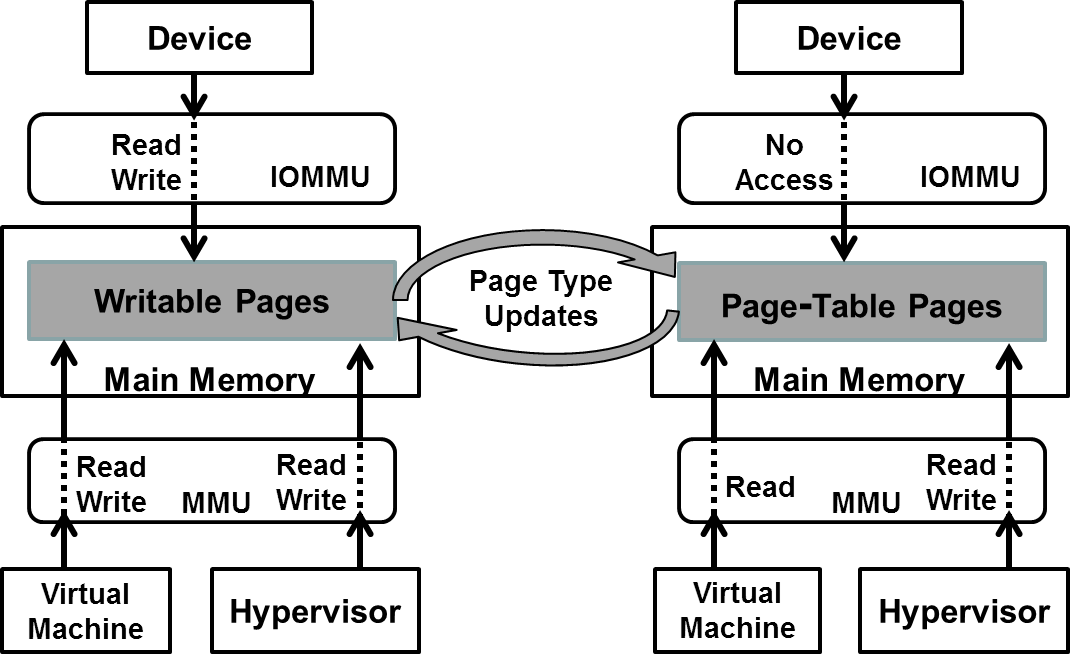
\includegraphics[width=0.5\textwidth]{image/background/wr2pt.png} \\
\caption{Page Type Updates With Safe Flag}
\label{fig:safe-flag}
\end{figure}

The modification to Xen is slight. Specifically, \name plans to use a redundant bit to represent the new flag to be compatible with its original design. However, in a 32-bit field related to page type information, each bit in the upper 9-bit has its specific use while the lower 23-bit serves as the reference count of current page type, representing at most ($2^23-1$) reference counts of the page type. It is reasonable for safe flag to occupy the top bit of the 23-bit as \name enforces a stricter rule to prevent count overflow.

\subsection{Cache Algorithm}
%secondly, design the cache pool to support it



enforce security polices in two aspects, i.e., guest OS and assigned I/O devices.Because of that, we associates the ready flag with

writable pages are writable for both guest OS and assigned I/O devices while

, , and  We defines that a writable page with a flag called \textbf{ready} that can be write-accessed by OS while inaccessible to devices. Because of that, when OS writes its writable pages with the ready flag (ready writable pages) as new page tables and submits the request of updating page tables, Xen reuses the existing validation process, however will not have to unmap them from I/O page tables instead the \textbf{ready} flag is marked with the page-table pages (ready page-table pages), thus reducing IOTLB-flushes. Besides, since the definition of page type is transparent to the OS, it needs to build a cache pool especially for the ready writable pages rather than free them into the buddy system which reserves only writable pages. Also, this cache mechanism benefits time efficiency when.

while provides every level of page-table cache pool for guest OS
